\documentclass{article} % For LaTeX2e
\usepackage{iclr2016_conference,times}
\usepackage{hyperref}
\usepackage{url}
\usepackage{graphicx}
\usepackage{tikz}
\usetikzlibrary{matrix}


\title{Build a Isolation Game Playing Agent\\
       AI Nanodegree Project Report}


\author{Veeresh Taranalli \\
\texttt{veeresht@gmail.com}
}

% The \author macro works with any number of authors. There are two commands
% used to separate the names and addresses of multiple authors: \And and \AND.
%
% Using \And between authors leaves it to \LaTeX{} to determine where to break
% the lines. Using \AND forces a linebreak at that point. So, if \LaTeX{}
% puts 3 of 4 authors names on the first line, and the last on the second
% line, try using \AND instead of \And before the third author name.

\newcommand{\fix}{\marginpar{FIX}}
\newcommand{\new}{\marginpar{NEW}}

%\iclrfinalcopy % Uncomment for camera-ready version

\begin{document}


\maketitle

% \begin{abstract}
% The abstract paragraph should be indented 1/2~inch (3~picas) on both left and
% right-hand margins. Use 10~point type, with a vertical spacing of 11~points.
% The word \textsc{Abstract} must be centered, in small caps, and in point size 12. Two
% line spaces precede the abstract. The abstract must be limited to one
% paragraph.
% \end{abstract}

% ==============================================================================
\section{Introduction}
\label{sec:intro}

In this project, we develop an AI agent for playing the game of Isolation. Isolation is a two-player game played on a rectangular grid of positions where both players take turns to move their piece and the first player who runs out of available moves loses the game. The positions occupied in previous moves are blocked for all future moves and in this specific version of Isolation game, the pieces are only allowed to move in L-shaped steps, just like a knight on a Chess board.

The main objectives of this project are:
\begin{itemize}
    \item Implement Minimax algorithm for searching the game tree.
    \item Implement Alpha-Beta pruning to improve the efficiency of the minimax game tree search.
    \item Utilize Iterative Deepening (ID) along with the Alpha-Beta search to implement the Isolation game AI agent that returns the best next move within the
    time provided to it.
    \item Develop heuristic evaluation functions that perform comparably or better than the provided heuristic evaluation functions.
\end{itemize}

\section{Heuristic Evaluation Functions}
\label{sec:heuristics}

We propose three different heuristics in addition to the ones provided in the starter package for the project. The heuristic evaluation functions provided to us are described as follows:

\begin{itemize}
    \item Null Score: This function returns 0 for all game board states which are non-terminal states.
    \item Open Moves Score: This function returns the number of moves available to player in a given board state as the score for non-terminal states.
    \item Difference of Open Moves Score (Improved): This function returns the difference in the number of moves available to the player and the opponent player in a given board state as the score for non-terminal states.
\end{itemize}

The proposed heuristic evaluation functions are described as follows:

\begin{itemize}
    \item Weighted Open Moves (H1): The idea here is to modify the Open moves score heuristic provided to us by weighting each open move by a weight that depends on the position the move leads to on the game board. The motivation is that positions in the center of the board provide more open moves than those near the edges. The weight for a position is set as the maximum number of moves available from that position on the board as shown below for a $7 \times 7$ board.

    \begin{center}
    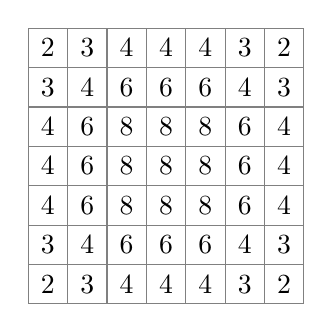
\begin{tikzpicture}
        \draw[step=0.5cm,color=gray] (-1,-1) grid (2.5,2.5);
        \node at (-0.75,+2.25) {2};
        \node at (-0.75,+1.75) {3};
        \node at (-0.75,+1.25) {4};
        \node at (-0.75,+0.75) {4};
        \node at (-0.75,+0.25) {4};
        \node at (-0.75,-0.25) {3};
        \node at (-0.75,-0.75) {2};

        \node at (-0.25,+2.25) {3};
        \node at (-0.25,+1.75) {4};
        \node at (-0.25,+1.25) {6};
        \node at (-0.25,+0.75) {6};
        \node at (-0.25,+0.25) {6};
        \node at (-0.25,-0.25) {4};
        \node at (-0.25,-0.75) {3};

        \node at (+0.25,+2.25) {4};
        \node at (+0.25,+1.75) {6};
        \node at (+0.25,+1.25) {8};
        \node at (+0.25,+0.75) {8};
        \node at (+0.25,+0.25) {8};
        \node at (+0.25,-0.25) {6};
        \node at (+0.25,-0.75) {4};

        \node at (+0.75,+2.25) {4};
        \node at (+0.75,+1.75) {6};
        \node at (+0.75,+1.25) {8};
        \node at (+0.75,+0.75) {8};
        \node at (+0.75,+0.25) {8};
        \node at (+0.75,-0.25) {6};
        \node at (+0.75,-0.75) {4};

        \node at (+1.25,+2.25) {4};
        \node at (+1.25,+1.75) {6};
        \node at (+1.25,+1.25) {8};
        \node at (+1.25,+0.75) {8};
        \node at (+1.25,+0.25) {8};
        \node at (+1.25,-0.25) {6};
        \node at (+1.25,-0.75) {4};

        \node at (+1.75,+2.25) {3};
        \node at (+1.75,+1.75) {4};
        \node at (+1.75,+1.25) {6};
        \node at (+1.75,+0.75) {6};
        \node at (+1.75,+0.25) {6};
        \node at (+1.75,-0.25) {4};
        \node at (+1.75,-0.75) {3};

        \node at (+2.25,+2.25) {2};
        \node at (+2.25,+1.75) {3};
        \node at (+2.25,+1.25) {4};
        \node at (+2.25,+0.75) {4};
        \node at (+2.25,+0.25) {4};
        \node at (+2.25,-0.25) {3};
        \node at (+2.25,-0.75) {2};
    \end{tikzpicture}
    \end{center}

    \item Difference in Weighted Open Moves (H2): In this heuristic, we calculate the difference in the weighted open moves scores (H1) between the current player and its opponent and use that as the score of the current game state.

    \item Difference in Open Moves One Ply Ahead (H3): The difference in the number of available moves between the current player and its opponent one ply ahead in the future is used as the score of the current game state.

\end{itemize}

\section{Results}
\label{sec:results}
The performance of the Isolation playing AI agents is evaluated using a tournament setup which consists of a Random AI agent that moves randomly and a set of AI agents utilizing minimax search (MM) and minimax with alpha-beta pruning (AB) search algorithms with fixed depth game trees as the opponents which use the Null, Open, Improved heuristic evaluation functions and the players includes agents that use iterative deepening (ID) with the Improved, H1, H2 and H3 heuristic evaluation functions.

To estimate and compare the performance of the proposed heuristic evaluation functions to the \mbox{ID-Improved} agent, we simulate 10 tournaments each consisting of 20 matches against every opponent for a particular heuristic evaluation function and another longer tournament consisting of 400 matches per opponent for a particular heuristic evaluation function as shown in Table~1 and Table~2 respectively. We observe that the ID-H3 player consistently performs better than all the other heuristics considered. The gain in performance is around 5\%.



\begin{table}[!ht]
    \caption{Table showing the results for all the ID agents with different
           heuristics in 10 tournaments each consisting of 20 matches per opponent.}
    \label{table_1}
    \centering
    \bgroup
	\def\arraystretch{1.5}%  1 is the default, change whatever you need
    \tabcolsep=0.11cm
    \begin{tabular}{|c|c|c|c|c|}
        \hline
        Tournament No. & ID-Improved & ID-H1 & ID-H2 & ID-H3 \\
        \hline
        1 & 76.43\% & 75.00\% & 82.14\% & 86.43\% \\
        \hline
        2 & 74.29\% & 74.29\% & 82.14\% & 76.43\% \\
        \hline
        3 & 77.14\% & 77.14\% & 75.71\% & 78.57\% \\
        \hline
        4 & 81.43\% & 77.86\% & 77.86\% & 79.29\%\\
        \hline
        5 & 77.86\% & 76.43\% & 77.14\% & 79.29\% \\
        \hline
        6 & 82.86\% & 73.57\% & 77.14\% & 85.00\% \\
        \hline
        7 & 76.43\% & 74.29\% & 79.29\% & 79.29\%\\
        \hline
        8 & 77.14\% & 78.57\% & 76.43\% & 77.86\% \\
        \hline
        9 & 74.29\% & 75.00\% & 78.57\% & 80.71\%\\
        \hline
        10 & 80.00\% & 74.29\% & 81.43\% & 77.86\% \\
        \hline
        Mean & 77.79\% & 75.64\% & 78.79\% & 80.07\% \\
        \hline
        Std. Dev. & 2.70\% & 1.64\% & 2.26\% & 3.04\% \\
        \hline
    \end{tabular}
    \egroup
\end{table}

\begin{table}[!ht]
    \caption{Table showing the results for all the ID agents with different
           heuristics in a tournament consisting of 400 matches per opponent.}
    \label{table2}
    \centering
    \bgroup
	\def\arraystretch{1.5}%  1 is the default, change whatever you need
    \tabcolsep=0.11cm
    \begin{tabular}{|c|c|c|c|c|c|c|c|c|}
        \hline
            & Random & MM-Null & MM-Open & MM-Improved & AB-Null & AB-Open & AB-Improved & Win \% \\
        \hline
        ID-Improved & 369 to 31 & 348 to 52 & 292 to 108 & 284 to 116 & 322 to 78 & 269 to 131 & 262 to 138  & 76.64\% \\
        \hline
        ID-H1 & 377 to 23 & 344 to 56 & 303 to 97  & 278 to 122 & 326 to 74 & 287 to 113 & 269 to 131 & 78.00\% \\
        \hline
        ID-H2 & 382 to 18 & 356 to 44 & 306 to 94 & 317 to 83 & 316 to 84 & 290 to 110 & 277 to 123 & 80.14\% \\
        \hline
        ID-H3 & 372 to 28 & 362 to 38 & 333 to 67 & 315 to 85 & 325 to 75 & 291 to 109 & 281 to 119 & 81.39\% \\
        \hline
    \end{tabular}
    \egroup
\end{table}

The H3 heuristic evaluation function is recommended to be used and can be justified as follows:
\begin{itemize}
    \item The H3 heuristic is based on the number of moves looking ahead one ply in the future. This is important in this version of isolation where only L-shaped knight like moves are allowed.
    Due to these kinds of moves, its difficult to predict the value of a game state by just counting the number of immediately available moves like in the Improved heuristic. Hence one ply lookahead should provide a more accurate evaluation function.
    \item The H3 heuristic running time complexity is comparable to the Improved heuristic and hence it should not adversely affect the maximum depth searched.
    \item As noted from the results, the H3 heuristic does perform better in practice and hence can be recommended.
\end{itemize}


% ==============================================================================

%\subsubsection*{Acknowledgments}

% ==============================================================================
% \bibliography{references}
% \bibliographystyle{iclr2016_conference}

\end{document}
